\section{Occupancy Problems}
Betragt følgende eksperiment: Vi har $n$ bins og $m$ balls, og smider hver ball i en uniformt tilfældig bin. Balls'ne smides i bins uafhængigt af hinanden. Med $n = 5$ og $m = 4$ kunne det eksempelvis ende sådan her:

\begin{figure}[H]
  \begin{center}
  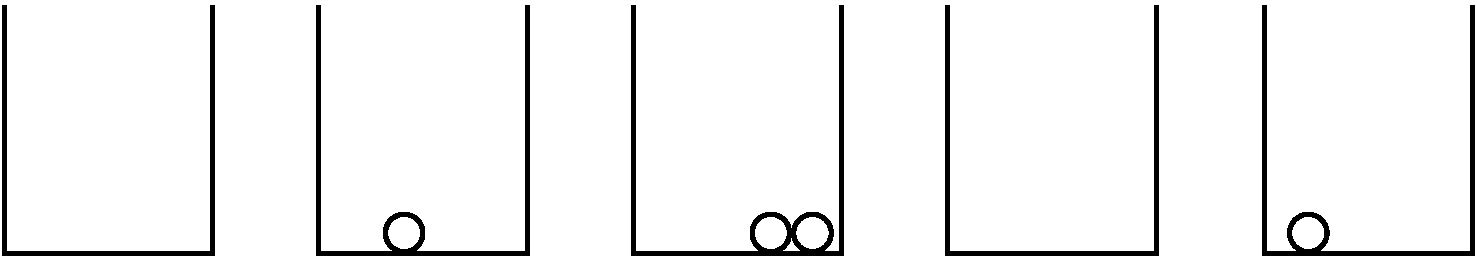
\includegraphics[width=\textwidth]{bins.pdf}
  \end{center}
  \caption{Eksempel på endt eksperiment}
  \label{fig:bins}
\end{figure}


Vi ønsker nu at besvare to forskellige spørgsmål; henholdsvis hvad sandsynligheden for, at ingen bin har mere end $k^\ast$ balls og hvad sandsynligheden for 0 kollisioner er.

\subsection{Sandsynlighed for at ingen bin har mere end $k^\ast$ balls}
Lad os antage, at $n = m$, altså at vi har lige mange bins og balls. Lad os starte med at betragte bin nr. $i \in \{ 1, ..., n \}$ og definere følgende to events:
\begin{align*}
  \event_i^{=k}:& \text{ Bin $i$ modtager præcis $k$ balls}\\
  \event_i^{\geq k}:& \text{ Bin $i$ modtager $\geq k$ balls}
\end{align*}

Lad os starte med at beregne sandsynligheden for $\event_i^{=k}$. Det må svare til sandsynligheden for, at den ene bold vi kaster i hver iteration rammer ned i præcis bin $i$ ud af alle $n$ bins, og gør det $k$ gange $(1/n)^k$, og i alle de resterende kast $n-k$ at de ikke ryger ned i denne bin $(1 - 1/n)^{n-k}$.\\
Herudover skal vi tage højde for, at der er $\binom{n}{k}$ måder at gøre det på, da vi er ligeglad med rækkefølgen boldene ryger i:
\begin{align}
  \P{\event_i^{=k}} &= \binom{n}{k} \pfrac{1}{n}^k \p{1 - \frac{1}{n} }^{n-k} \label{eq:event-i-lig-k} \\
  &\leq \pfrac{ne}{k}^k \pfrac{1}{n}^k \label{eq:prop-b.2.3} \\
  &= \pfrac{e}{k}^k \label{eq:res-bestemt-k}
\end{align}

Hvor vi i \cref{eq:prop-b.2.3} bruger Proposition B.2.3, nemlig at såfremt $n \geq k \geq 0$ (hvilket vi antager gælder), så har vi, at $\binom{n}{k} \leq \pfrac{ne}{k}^k$. Derudover kan vi fjerne $(1 - 1/n)^{n-k}$ fra \cref{eq:event-i-lig-k} (for at gøre vores udtryk nemmere at regne på), da vi ved at det vil være $\leq 1$.


Lad os nu beregne sandsynligheden for $\event_i^{\geq k}$. Det må svare til:
\begin{align}
  \P{ \event_i^{\geq k} }
  &= \P{ \bigcup_{k' = k}^n \event_i^{=k'} } \nonumber \\
  &\leq \sum_{k=k'}^n \P{ \event_i^{=k'} } \label{eq:prob-union-bound} \\
  &\leq \sum_{k=k'}^n \pfrac{e}{k'}^{k'} \label{eq:benyt-fundne} \\
  &\leq \sum_{k=k'}^n \pfrac{e}{k}^{k'} \label{eq:mindre-k} \\
  &= \pfrac{e}{k}^k \p{ 1 + \pfrac{e}{k} + \pfrac{e}{k}^2 + \cdots + \pfrac{e}{k}^{n-k} } \label{eq:e-k-uden-for-parentes} \\
  &\leq \pfrac{e}{k}^k \sum_{i = 0}^\infty \pfrac{e}{k}^i \nonumber \\
  &= \pfrac{e}{k}^k \frac{1}{1 - \frac{e}{k}} \label{eq:endelig-res}\\
  &= O(n^{-2}) \quad \text{(*Givet en bestemt $k$-værdi)} \label{eq:prob-til-O}
\end{align}

I \cref{eq:prob-union-bound} benytter vi union bound.\\
I \cref{eq:benyt-fundne} benytter vi vores udtryk bestemt i \cref{eq:res-bestemt-k}.\\
I \cref{eq:mindre-k} benytter vi, at $k \leq k'$ for de forskellige $k'$, så brøken kan kun potentielt blive større.\\
I \cref{eq:e-k-uden-for-parentes} sætter vi $\pfrac{e}{k}^k$ uden for en parentes, og benytter herefter potensregneregler til at gange ind hvorved vi får samme sum som i ligningen før.\\
I \cref{eq:endelig-res} benytter vi en regneregel for en uendelig sum.\\
I \cref{eq:prob-til-O} vælger vi vores $k$ til
$$
k = \frac{c \, \ln n}{\ln \ln n}
$$
hvorved vi får vores resultat $O(n^{-2})$ for en passende konstant $c$. Udledningen for dette er ikke vigtig til eksamen, men kan ses i \nameref{subsec:udledningO} (værdien for $k$ er dog vigtig).\\\\


Vi har netop vist, at sandsynligheden for at præcis bin $i$ modtager $\geq k^\ast$ balls $\P{ \event_i^{\geq k^\ast} } \leq \frac{1}{n^2}$ for $i = 1, ..., n$.
Så vil sandsynligheden for at ingen af de $i \in \{1, ..., n\}$ forskellige bins modtager $\geq k^\ast$ balls være:
$$
\P{ \bigcup_{i=1}^n \event_i^{\geq k^\ast} }
\leq \sum_{i=1}^n \P{ \event_i^{k^\ast} }
\leq \sum_{i=1}^n \frac{1}{n^2}
= n \, \frac{1}{n^2}
= \frac{1}{n}
$$

Ud fra dette kan vi tydeligt se, at med sandsynlighed $\geq 1 - 1/n$ modtager hver bin færre end $k^\ast = \frac{c \ln n}{\ln \ln n}$ balls.

\newpage
\subsection{Sandsynlighed for 0 kollisioner}
Her antager vi \emph{ikke} at der nødvendigvis skal gælde, at $m = n$. Lad os definere event $\event_i$:\\
$\event_i$: Den $i$'te ball lander i en bin som er tom ved det $i$'te kasts begyndelse.


\begin{align}
  \P{\bigcap_{i=1}^m \event_i}
  &= \prod_{i=1}^m \, \P{\event_i \middle| \bigcap_{j=1}^{i-1} \event_j} \nonumber \\
  &= \prod_{i=1}^m \frac{n - (i-1)}{n} \label{eq:prob-ite-op} \\
  &= \prod_{i=1}^m \p{ 1 - \frac{i-1}{n} } \nonumber \\
  &\leq \prod_{i=1}^m e^{- \frac{i-1}{n}} \label{eq:1+x-regneregel} \\
  &= e^{ - \sum_{i=1}^m \frac{i-1}{n}} \nonumber\\
  &= e^{- \frac{1}{n} \sum_{i=1}^m (i - 1) } \label{eq:gange-n-udenfor} \\
  &= e^{- \frac{1}{n} \pfrac{(m-1)m}{2} }  \label{eq:sum-til-m}  \\
  &= e^{- \frac{(m-1)m}{2n}}  \label{eq:endelig-res-2}
\end{align}

I \cref{eq:prob-ite-op} benytter vi, at der i den $i$'te iteration er blevet udført $(i-1)$ kast, hvorved der må være $n - (i-1)$ bins tilbage der resulterer i succes, og der er $n$ mulige bins at ramme i alt.\\
I \cref{eq:1+x-regneregel} benytter vi regnereglen $1 + x \leq e^x$ for $x \in \R$.\\
I \cref{eq:gange-n-udenfor} ser vi, at vi kan gange $1/n$ udenfor summen.\\
I \cref{eq:sum-til-m} benytter vi det velkendte faktum, at $\sum_{i=1}^n = \frac{n(n-1)}{2}$.\\
I \cref{eq:endelig-res-2} ganger vi blot $1/n$ ind igen.\\

Herved finder vi, at for $m \geq \sqrt{2n} + 1$, så vil $\P{\bigcap_{i=1}^m \event_i} \leq e^{-1}$.


\subsubsection{Eksempel på benyttelse: Birthday problem}
Givet $m$ mennesker, hvor sandsynligt er det så at nogle af dem har fødselsdag på samme dag?\\

Vi har, at bins svarer til antal dage, og balls svarer til antal mennesker. Lad os sige vi har $m = \ceil{\sqrt{2n} + 1} = 29$ mennesker, hvor $n = 365$.\\

Da får vi:
$$
\P{\bigcap_{i=1}^m \event_i} \leq 0.329
$$

Altså er sandsynligheden for, at ingen har fødselsdag samme dag bestemt til $\leq$ 33 \%.
